%
% LaTeX template for EEE MSc Dissertation
% Available for all PGT & PGR students at the UoM
% v2.0 released 03 August 2020
% Authors:
% Farshad Arvin & Alex Casson

% Change log
% v1.0 June 2020
%    Beta testing only - never publicly released
%    A few minor margin changes & Calibri Fonts
%    First version: a simple template for MSC Dissertation
%============================================

\documentclass[12pt]{article}
\usepackage{graphicx}
\usepackage{fontspec}
\usepackage[utf8]{inputenc}
\usepackage[english]{babel}

%================ Font
% Calibri Font
\setromanfont[
BoldFont=CalibriBold.ttf,
ItalicFont=CalibriItalic.ttf,
BoldItalicFont=CalibriBoldItalic.ttf,
]{Calibri.ttf}
%=============== Margin
\usepackage{geometry}
\geometry{a4paper, left=22mm,  top=22mm, bottom=22mm, right=22mm}
%===============
\usepackage{setspace}
\usepackage[document]{ragged2e} % left-alignment
\hyphenpenalty=10000
\tolerance=10000
%--------------------------------
\begin{document}
\onehalfspacing
%========= Title Page
\thispagestyle{empty} 
\begin{titlepage}
    \centering
    
\includegraphics[width=0.25\textwidth]{uom_logo.pdf}
    \hspace{170}
    
\includegraphics[width=0.35\textwidth]{Sheffield.pdf}
    \begin{center}
       \vspace*{4cm}
       {\LARGE Research Software Engineering Practice}
       \vspace{3cm}
    \begin{large}   
    

         
         \vspace{0.5cm}

        {\LARGE Analysis of the connectivity of hydrides within the microstructure of Zr alloys} \\

       \vspace{1.5cm}
        
        {\bf \today} \\
                
        
       \vspace{3 cm}
        Group 2 \\
       \textbf{Laura Gonzalez,
       Wunmi Olukoya,
       Jamie McGregor, 
       Enn Veikesaar }\\

       \vfill
       \centering
       
        {\bf \large Advanced Metallic System CDT Program}\\
          
        
\includegraphics[width=0.35\textwidth]{CDT.jpg}
        
    
    
    \end{large}  
   \end{center}
\end{titlepage}
%========= Abstract
\newpage 
\thispagestyle{plain} 
\pagenumbering{roman}
\section*{Summary}
     This LaTeX template was prepared for the UoM PGR Final Dissertation.
     
%========== Table of Content
\newpage
\begin{singlespacing}
\tableofcontents
\end{singlespacing}
\setlength{\parskip}{1em}
\renewcommand{\baselinestretch}{2.0}

%>>>>>>>>>>>>>>>>>>>>>>>>>>>>>>>>>>>>>>>>
% Main body of Thesis
%========= Start of the report
\newpage 
\pagenumbering{arabic}
\setcounter{page}{1}
\onehalfspacing

%========= Contributions
\section{Contributions}

Description of each team members role and contribution

Laura Gonzalez:
Wunmi Olukoya:
Jamie Mcgregor: 
Enn Veikesaar:




%========= Introduction
\section{Introduction}

\subsection{The presence of hydrides in Zr-alloys}

\justify
\noindent
Zr alloys are widely employed as fuel cladding in the nuclear sector. When corrosion occurs in nuclear reactors, the released hydrogen penetrates into the cladding alloy. This material absorbs part of it but, once the solubility limit is reached, hydrogen precipitates into brittle hydrides platelets. Generally, the hydrides orient along the tube circumferential direction, but they may orient radially too. Cladding usually fails by a hoop stress, so radial hydrides will lead the alloy to fail earlier in deformation processes. Moreover, crack propagation through cladding thickness is alarming, and this occurrence will be especially facilitated by radial-oriented hydrides. As cladding alloys fail more easily under the presence of radial hydrides, it is important to study the changes in hydride orientation to control cladding embrittlement \cite{SIMON2021152817, COLAS2013586, SHARMA2018546, SUNIL2020152457}.

\noindent
Cladding failure under hoop stress is strongly  affected by these three factors:

\vspace{0.1 mm}
- Hydrogen and hydride content.

\vspace{0.1 mm}
- Fraction of radially-oriented hydrides.

\vspace{0.1 mm}
- Continuity in the hydrides along the thickness of the cladding \cite{SIMON2021152817}.

\noindent
To measure the two last factors, parameters as the Radial Hydride Fraction (RHF), the Hydride Continuity Coefficient (HCC) and the Radial Hydride Continuity Factor (RHCF) are used. The RHF, always between 0 and 1, represents the fraction of radially-oriented hydrides. Higher values of this parameter are related to more propagation of the cracks through the cladding thickness. But some microstructures with different hydrides locations may have the same RHF value in some cases, as it is shown in Figure 1. Therefore, it is also necessary to measure the continuity the hydrides, as this variable has an important effect on crack propagation. The HCC and RHCF determine how close the hydride platelets are to each other and show radial hydrides alignment across the cladding thickness, which is related to cracking propagation through the cladding thickness. These parameters, generally between 0 and 1, the higher they are, the more connected the hydrides across the thickness of the material will be \cite{SIMON2021152817}, which leads to the material's embrittlement.

\vspace{50 mm}

\begin{figure}[h] %  figure placement: here, top, bottom, or page
    \centering
    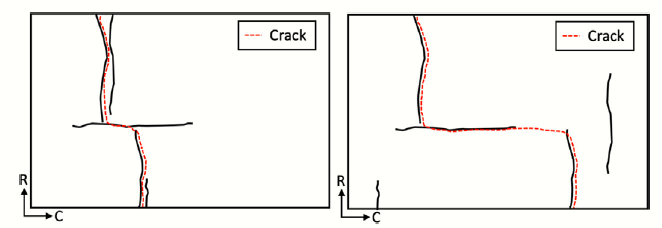
\includegraphics[width=4.3in]{same RHF.png}
    \caption{Same hydrides located differently: The same RHF value but different alignment \cite{SIMON2021152817}.}
    \label{fig:my_label}
\end{figure}

\subsection{Parameters calculation}


\noindent
RHF corresponds to the weight average of hydride length multiplied by a weighting factor. The formula employed is described below:

\begin{figure}[h] %  figure placement: here, top, bottom, or page
    \raggedleft
    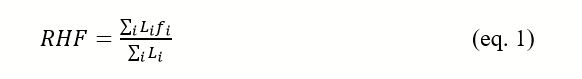
\includegraphics[width=4.3in]{RHF.JPG}
    \label{fig:my_label}
\end{figure}


\noindent
Where $L_i$ is the length of each hydride and $f_i$ is the weighting factor, a parameter that has different values depending on the hydrides orientation. Hydrides with orientations between 0-40° to the transverse direction have a $f_i$ of 0, when the orientation is between 40° and 65°, the $f_i$ is 0.5, and hydrides with an orientation of 65–90° have a $f_i$ of 1 \cite{COLAS2013586}. 

\noindent
To calculate the HCC, a rectangular area in the micrograph of the alloy is separated, and the length of each radial hydride in that area is measured. The formula applied is shown below:


\begin{figure}[h] %  figure placement: here, top, bottom, or page
    \raggedleft
    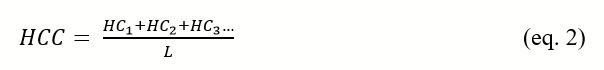
\includegraphics[width=4.3in]{HCC.JPG}
    \label{fig:my_label}
\end{figure}
\noindent
Where $HC_i$ is the length of each radial hydride and L is the height of the selected rectangle to measure \cite{SIMON2021152817}.

\noindent
To calculate the RHCF, the length of each radial hydride in a section of the cladding is measured. This time, the section will have a length of 150 µm along the arc length of the cladding, and the width will be all the cladding thickness. The formula applied in this case is:

\begin{figure}[h] %  figure placement: here, top, bottom, or page
    \raggedleft
    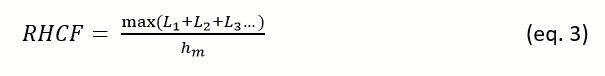
\includegraphics[width=4.5in]{RHCF.JPG}
    \label{fig:my_label}
\end{figure}

\vspace{150}
\noindent
Where $L_i$ is the length of each radial hydride within the 150 µm of arc length, and $h_m$ is the cladding thickness \cite{SIMON2021152817}.

\subsection{Limitations of each parameter}

\noindent
The problem of the RHF is that it does not differentiate between hydrides oriented within the ranges 0-40°, 40-65°, and 65-90° \cite{SIMON2021152817}. Thus, microstructures with different radial hydrides orientations can have the same $f_i$, which will lead to obtain the same value of RHF.

\noindent
The continuity factors do not differentiate some situations either. For example, the HCC is the same in the three situations illustrated in Figure 2, which certainly facilitate the cracking propagation to different extents. In Figure 3 it can be seen that two different situations entail the same value of RHCF and, on the contrary, Figure 4 shows how two equivalent situations may lead to different values of RHCF \cite{SIMON2021152817}.

\begin{figure}[h] %  figure placement: here, top, bottom, or page
    \centering
    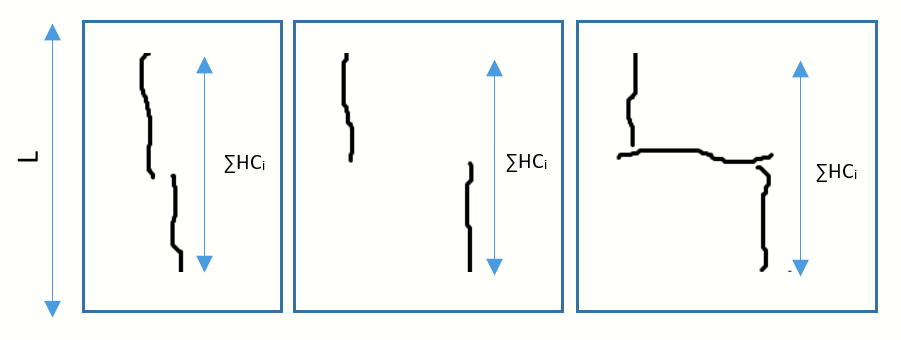
\includegraphics[width=4.5in]{HCC comparison.png}
    \caption{Radial-oriented hydrides differently located but with the same HCC value.}
    \label{fig:my_label}
\end{figure}

\begin{figure}[h] %  figure placement: here, top, bottom, or page
    \centering
    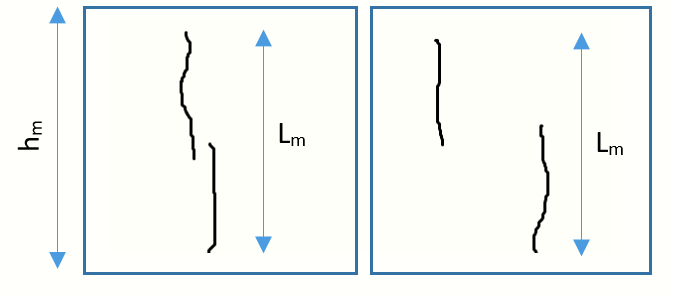
\includegraphics[width=4.5in]{RHCF comparison 1.png}
    \caption{Radial-oriented hydrides with the same RHCF value but different connectivity.}
    \label{fig:my_label}
\end{figure}

\begin{figure}[h] %  figure placement: here, top, bottom, or page
    \centering
    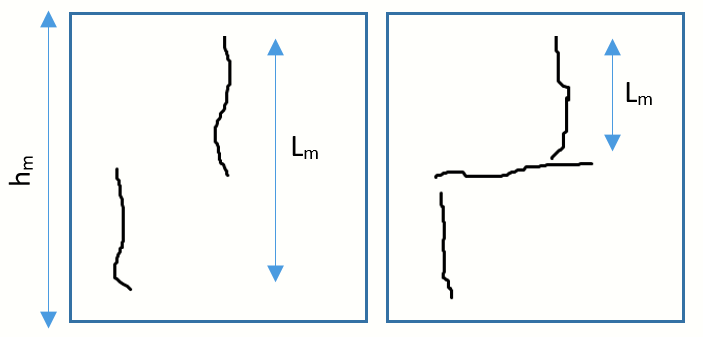
\includegraphics[width=4.5in]{RHCF comparison 2.png}
    \caption{Radial-oriented hydrides with the different RHCF value but the same connectivity.}
    \label{fig:my_label}
\end{figure}


%========= Literature review
\section{Literature review}

Small Literature survey of the existing methods of connectivity determination

\cite{COLAS2013586}
\cite{SHARMA2018546}
\cite{SUNIL2020152457}

%========= Methodology
\section{Methodology \& Discussion}

In this work, three types of thresholding was performed: Otsu, K-mean and Gaussian. The HCC was calculated for all of them to check which method is the most accurate in terms of hydrides connectivity evaluation. Using GitHub to collaborate, we developed a Jupyter notebook were many functions are called to show clarity in the script.

The following sections were developed throughout the workflow:

\begin{enumerate}

    \item \textbf{Import packages.}
This sections is used to  call all the packages needed to the correct running of the whole script.

    \item\textbf{ Import the images from GitHub.}
In this part of the code, the images to analyse are loaded.

    \item \textbf{Image processing.}
Because of the large area of the images being analysed, there are shadows that may lead us to incorrect results. To solve this, here it is included some code to break the image into vertical grayscale strips. The strips are also blurred and saved in their own directories.

    \item \textbf{Thresholding.}
In this part, the grayscale and blurred strips are transformed into binary images and three different thresholding methods are applied to see which one offers the best result.
o	Otsu thresholding
o	K-means thresholding
o	Gauss thresholding

    \item \textbf{Connectivity of microstructure.}
In this section, the connectivity between hydrides in the radial direction is checked and the edges are detected to discover the contours within the slices. With this information, the HCC parameter of each strip is measured, and finally the average HCC value is obtained for each of the three thresholding methods.
\end{enumerate}

\section{Results \& Discussion}


%========= Conclusions
\section{Conclusions \& Future Work}



%>>>>>>>>>>>>>>>>>>>>> End of Thesis 

%-------- Bibliography
\newpage
\singlespacing
\bibliography{biblography}
\bibliographystyle{IEEEtran}
\end{document}